\documentclass[tikz]{standalone}
\usepackage{amsmath,amssymb}
\usepackage{pgfplots,multicol}

\pgfplotsset{compat=1.10}
\usepgfplotslibrary{fillbetween}

\begin{document}



 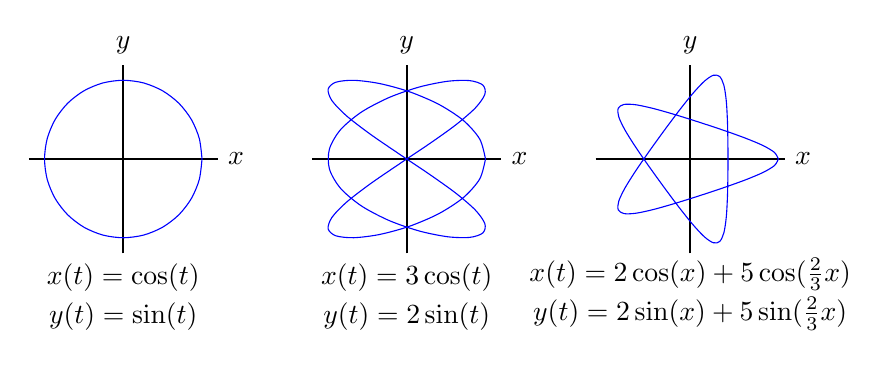
\begin{tikzpicture}[xscale=0.2,yscale=0.2]
        \draw[-,thick] (-6,0) -- (6,0) node[right] {$x$};
         \draw[-,thick] (0,-6) -- (0,6) node[above] {$y$};

	
	\draw[-,smooth,domain=0:360,blue] plot({5*cos(\x)},{5*sin(\x)});
	

	\draw[fill=black] (0,-9) node[above] {$x(t)=\cos(t)$};
	\draw[fill=black] (0,-11.5) node[above] {$y(t)=\sin(t)$};
	
	 \draw[-,thick] (12,0) -- (24,0) node[right] {$x$};
         \draw[-,thick] (18,-6) -- (18,6) node[above] {$y$};
	\draw[-,smooth,domain=0:360,blue,samples=50] plot({5*cos(3*\x)+18},{5*sin(2*\x)});
	\draw[fill=black] (18,-9) node[above] {$x(t)=3\cos(t)$};
	\draw[fill=black] (18,-11.5) node[above] {$y(t)=2\sin(t)$};


	 \draw[-,thick] (30,0) -- (42,0) node[right] {$x$};
         \draw[-,thick] (36,-6) -- (36,6) node[above] {$y$};
	\draw[-,smooth,domain=0:1080,blue,samples=50] plot({0.8*(2*cos(\x)+5*cos(2/3*\x))+36},{0.8*(2*sin(\x)-5*sin(2/3*\x))});
	\draw[fill=black] (36,-9) node[above] {$x(t)=2\cos(x)+5\cos(\frac{2}{3}x)$};
	\draw[fill=black] (36,-11.5) node[above] {$y(t)=2\sin(x)+5\sin(\frac{2}{3}x)$};





\end{tikzpicture}


	
\end{document}
